\section{Introduction}

\begin{figure}[t]
\centering
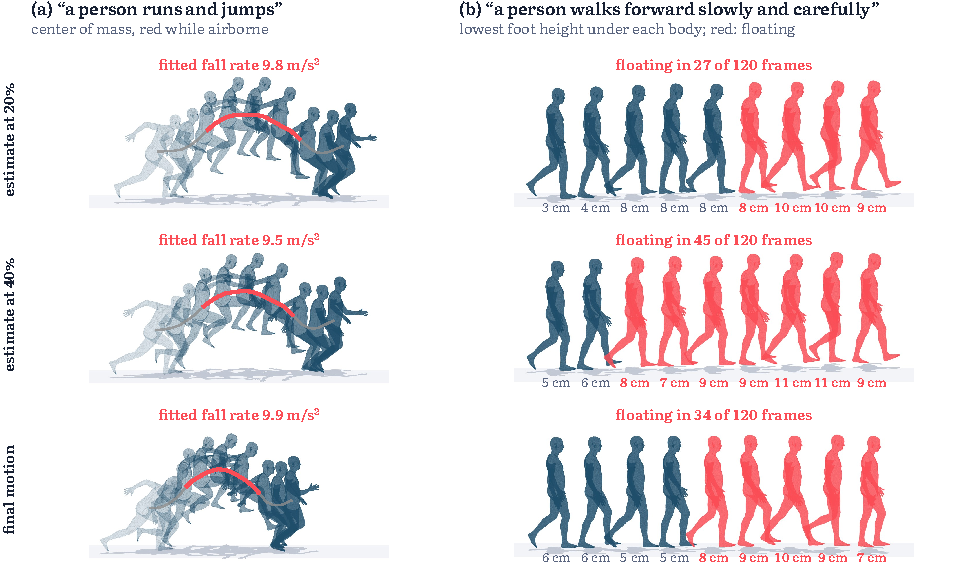
\includegraphics[width=\linewidth]{figures/web/fig_teaser.pdf}
\caption{The model's own clean-motion estimate already shows the physics of the final motion. Views from the side and slightly above of two recorded samples from the 50-step MDM, drawn from its clean-motion estimate at 20\% and 40\% of denoising (top and middle rows) and from the final motion (bottom row). (a) A jump: the center of mass (line, red while airborne) already follows a ballistic arc at 20\%; the fitted fall rate is printed above each row. (b) A slow walk that floats: red poses lie in floating stretches (airborne for at least 0.2\,s with a fitted fall rate below 2\,m/s$^2$), and the numbers give the lowest foot's height. The estimate at 20\% already floats where the final motion does. Poses in (b) are spread horizontally for readability. Bodies are SMPL meshes \citep{loper2015smpl} fitted to the generated joints for display \citep{bogo2016keep}, with a mean joint error of 1.0 to 1.2\,cm; shadows are vertical projections onto the floor. Every number in the figure is computed from the joints.}
\label{fig:teaser}
\end{figure}

Text-to-motion models turn a sentence into seconds of fluent human movement \citep{guo2022humanml3d,tevet2023mdm,zhang2023t2mgpt,guo2024momask,rempe2026kimodo}. Most are kinematic. They output joint positions and rotations directly, with no simulator, so whatever physics they produce is learned from motion capture and never enforced. Physics-based generators instead move a simulated character, so gravity and contact hold by construction \citep{peng2018deepmimic,tessler2024maskedmimic}. Kinematic models' most visible failures are therefore physical: bodies hover above the ground, feet slide while planted, and jumps do not fall as they should. Most remedies act from outside the generator. They project samples through a physics simulator \citep{yuan2023physdiff}, condition on physical parameters \citep{simdiff2025}, model contact and body forces explicitly \citep{xing2026interphys}, or optimize the sampling noise \citep{physiblemdm2026}. Whether the generator itself represents the physics it gets wrong is a separate and useful question: if the physics is present inside the model but lost on the way out, the internal signal could flag failing samples before compute is spent finishing them.

For video diffusion models, recent work answers yes. Physical quantities are linearly decodable from transformer activations and are reported to be built inside the model rather than inherited from its input \citep{kneifl2026physics}. Plausibility is decodable from the internal states of models whose outputs violate physics, a finding its authors summarize as models that ``know more than they show'' \citep{esmati2026invisible}. Probes on denoising features are used to prune implausible samples early \citep{tang2026seeking}.

These conclusions rest on a comparison between a probe on internal activations and a readout of what the model takes in or puts out. In a diffusion model, the estimate of the clean sample at each step is computed from the activations at that step together with the noisy input (and, in MotionDiffuse, the text), so it cannot carry information about the outcome that they lack (Section~\ref{sec:fair}). A probe that beats a readout of the estimate shows only that the information is easier for that probe to use in the activations \citep{xu2020vinfo}. The output may still contain all of it. How much such a gap means depends on three things: whether the two readouts are equally flexible and equally well tuned; whether the gap holds within a prompt, or only reflects which prompt was given; and whether there was enough training data for the comparison to be stable.

We set out to show that a motion diffusion model, too, knows more than it shows, and to use that knowledge to stop failing samples early. Text-to-motion diffusion suits the test, because all three conditions can be checked: the physics of a motion follows exactly from its joint positions, the models we study expose a clean-motion estimate at every step (MDM predicts it, \citealp{tevet2023mdm}; MotionDiffuse computes it from its noise prediction, \citealp{zhang2022motiondiffuse}), and sampling is cheap enough to record thousands of complete trajectories. We record every transformer layer along each model's own sampling path, for 6,000 motions from 250 prompts with two MDM checkpoints and 3,000 with MotionDiffuse, and compute dynamic balance (the extrapolated center of mass relative to the area of foot support; \citealp{hof2005condition}), flight, gravity during flight, and floating from the final motions. Two choices were made along the way. We added a set of jump-heavy prompts once it was clear that the main prompts contain too few falling bodies to test gravity, and we redefined ``airborne'' after finding that the first definition counted hovering and crawling as flight (Appendix~\ref{app:labelfix}). The result is not the one we set out to show.

\paragraph{Contributions.}
\begin{itemize}
    \item \textbf{Physics is readable early.} A fifth of the way through denoising, linear probes on the layers already recover the final motion's dynamic balance and flight ($R^2 = 0.84$ and AUC 0.97 on the 50-step model), stably across seeds and on held-out prompts (Section~\ref{sec:readable}).
    \item \textbf{The apparent hidden knowledge is a readout effect.} Standard baselines make the layers look better informed than the estimate. Read with equal care, the estimate matches them. For balance and flight, on all three models, adding a layer gains at most 0.01, and a positive control shows that the protocol would detect a gain of that size. Floating behaves the same on the jump prompts; only in the smaller main data sets does the layer help (Section~\ref{sec:fairresults}). With too little training data the comparison can flip, which explains a pilot study that pointed the other way (Section~\ref{sec:learning}).
    \item \textbf{One exception, and it fades.} Only for the fall rate of jumps do the layers know more. A fifth of the way through denoising, MDM's layers add about 0.08 in $R^2$ (up to 0.11 in a refit) to the best readout of the estimate, and on the 50-step model the gain survives every control we applied. It fades as sampling proceeds and the estimate catches up. On MotionDiffuse the same gain is small and not robust (Section~\ref{sec:fairresults}).
    \item \textbf{The output is enough for early warning.} Decoded partway through sampling, MDM's own estimate flags samples that will float, without training and about as well as a trained probe on the layers. Aborting them saves under a tenth of the compute, because floating affects only 9 to 18\% of samples and concentrates in a few prompts (Section~\ref{sec:early}).
    \item \textbf{A related issue in video.} A linear probe at chance is the main evidence that plausibility is absent from the clean VAE latent of a video diffusion model \citep{esmati2026invisible}. One fixed, training-free nonlinearity, the size of local frame-to-frame change, makes it readable from the same latent: a linear readout of it reaches 78\% pairwise accuracy on IntPhys, and 80\% together with the grid features (Section~\ref{sec:video}).
    \item \textbf{What actually fails.} Once bodies that hover without falling are separated out, MDM's jumps fall at close to the right rate in the median. The common failure is floating, and on test captions the original 1000-step checkpoint floats about twice as often as the 50-step one (Section~\ref{sec:physics}).
\end{itemize}
Section~\ref{sec:discussion} turns these findings into five checks for probing studies that claim a generator knows more than it shows.
